\documentclass[a4paper,notitlepage]{article}

\usepackage{xltxtra}
\usepackage{amsmath}
\usepackage{amssymb}
\usepackage{amsthm}
\usepackage{tikz}
\usepackage{unicode-math}
\usepackage{fontspec}
\setmathfont{xits-math.otf}

\tikzset{node distance=2.5cm,auto}

\author{Víctor López Juan}
\title{Chapter 3}

\begin{document}


  \maketitle
\begin{enumerate}
  
  \item[9.]
{\em Complete the proof of Proposition 3.24 in the text by showing that $\bar{h} = h \circ i$ is indeed a homomorphism.}

    \begin{proof}
    \begin{itemize}
      Monoid homomorphisms must map identity elements to each other,
      and preserve the operation.
      
      \item

        $\bar{h}$ respects the unit element.
        
        \begin{align*}
         \bar{h}(1_M) &= h(i(1_M))                \tag{definition of $\bar{h}$} \\
                     &= h(\langle 1_M \rangle)                         \tag{definition of $i$} \\
                     &= h(μ(\langle \langle \rangle \rangle))           \tag{definition of $μ$} \\
                    &= h(ε(\langle \langle \rangle \rangle))           \tag{$h \circ μ = h \circ ε$} \\
                    &= h(\langle \rangle)                              \tag{definition of $ε$} \\
                    &= 1_N                                              \tag{$h$ is an homomorfism} \\
        \end{align*}

      \item

        $\bar{h}$ respects the monoid operation.

        \begin{align*}
           \bar{h}(xy) &= h(i(x·y))                                         \tag{definition of $\bar{h}$} \\
         &= h(\langle x·y \rangle)                            \tag{definition of $i$}  \\
         &= h(μ(\langle \langle x, y \rangle \rangle))        \tag{definition of $μ$} \\
         &= h(ε(\langle \langle x, y \rangle \rangle))        \tag{$h \circ μ = h \circ ε$} \\
         &= h(\langle x, y \rangle))                       \tag{definition of $ε$} \\
         &= h(\langle x \rangle \cdot \langle y \rangle)      \tag{definition of the free monoid} \\
         &= h(\langle x \rangle) \cdot h(\langle y \rangle)  \tag{$h$ is an homomorfism} \\
         &= h(i(x)) \cdot h(i(y))                                    \tag{definition of $i$} \\
         &= \bar{h}(x) \cdot \bar{h}(y)                              \tag{definition of $\bar{h}$} \\
         \end{align*}

     \end{itemize}
    \end{proof}

  \item[10.]

    {\em In the proof of Proposition 3.24 in the text it is shown that any monoid
     $M$ has a specific presentation $T^2 M \rightrightarrows T M → M$ as a coequalizer of free
     monoids. Show that coequalizers of this particular form are preserved by
     the forgetful functor $U : \text{\bf Mon} → \text{\bf Sets}$}

        Let $(\pi,M)$ be the coequalizer of $μ$ and $ε$, and $U$ be the
        forgetful functor $\text{\bf Mon} → \text{\bf Sets}$.

        We want to prove that $(U(\pi) = \pi, U(M) = \vert M \vert)$ is also a coequalizer in {\bf Sets}.

        \begin{proof}

        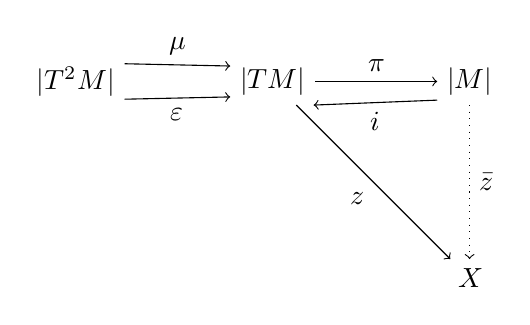
\begin{tikzpicture}
          \node (TTM) {$\vert T^2 M \vert$};
          \node (TM) [right of=TTM] {$\vert T M \vert$};
          \node (M)  [right of=TM]  {$\vert M \vert$};

          \node (X)  [below of=M]   {$X$};

          \draw[->] (TTM.20) to node {$μ$} (TM.160);
          \draw[->,swap] (TTM.340) to node {$ε$} (TM.200);
          \draw[->] (TM) to node {$\pi$} (M);
          \draw[<-,swap] (TM.330) to node {$i$} (M.210);

          \draw[->,swap] (TM) to node {$z$} (X);
          \draw[->,dotted] (M) to node {$\bar{z}$} (X);
        \end{tikzpicture}
        
        Let $i$ be the inclusion of generators into TM, $i : M → TM$,
        $i(x) = \langle x \rangle$.

        Let there be a set $X$, and an arrow $z : TM → X$ such that
        $z \circ μ = z \circ ε$. Then there's an arrow $\bar{z} : M → X$, $\bar{z} = z \circ i$,
        such that $\bar{z} \circ \pi = z$.

        \begin{align*}
          \bar{z}(\pi(\langle x_1, x_2, …, x_n \rangle))    &= \bar{z}(x_1 · … · x_n) \\
                                                           &= z(i(x_1 · … · x_n)) \\
                                                           &= z(\langle x_1 · … · x_n \rangle) \\
                                                           &= z(μ(\langle \langle x_1, …, x_n \rangle \rangle)) \\
                                                           &= z(ε(\langle \langle x_1, …, x_n \rangle \rangle)) \\
                                                           &= z(\langle x_1, …, x_n \rangle) \\
        \end{align*}

        To prove that this arrow unique in {\bf Set}, suppose
        $\bar{z}^\prime$ such that $\bar{z}^\prime \circ U(\pi) = z$.

        Then:

        \begin{align*}
          \bar{z}^\prime(x)   &= \bar{z}^\prime(U(\pi)(\langle x \rangle))  \tag{definition of $\pi$}\\
                            &= z(\langle x \rangle)                      \tag{hypothesis}          \\
                            &= \bar{z}(U(\pi)(\langle x \rangle))        \tag{property of $\bar{z}$}    \\
                            &= \bar{z}(x)                                \tag{definition of $\pi$}\\
        \end{align*}
 
        Therefore,

        $$\bar{z}^\prime = \bar{z}\text{ .}$$

        \end{proof}
\end{enumerate} 
\end{document}
   
 
